\section{Introduzione}
Il programma realizzato permette di gestire utenti e interventi di una squadra della Protezione Civile, utilizzando una semplice interfaccia grafica realizzata tramite il framework Qt.
In particolare, gli utenti sono suddivisi in base al loro ruolo:
\begin{itemize}
	\item volontario;
	\item caposquadra;
	\item amministratore.
\end{itemize}
Ogni utente, in base al proprio ruolo, avrà accesso a particolari funzionalità quali aggiungere o cancellare un utente nel sistema, visualizzare gli utenti della propria squadra, visualizzare e pianificare interventi. A differenza degli amministratori, il volontario e il caposquadra appartengono a una squadra, caratterizzata da un nome e da un'area di intervento. 
Per accedere all'applicazione è necessario effettuare un login, inserendo uno username, rappresentato dal proprio numero di matricola e una password scelta al momento della registrazione dell'utente.
L'interfaccia grafica è stata realizzata attraverso gli oggetti QtWidget che permettono di semplificare la realizzazione della GUI tramite l'editor Qt Creator.

\section{Funzionamento}
All'avvio del programma, viene subito richiesto di effettuare il login (\Fig\ref{fig:loginform}), inserendo lo username (costituito dalla matricola assegnata dal sistema al momento dell'inserimento dell'utente) e la password. In caso di username e/o password errati, viene mostrato un messaggio di errore e cancellati lo username e la password errati. Non è quindi possibile procedere oltre nell'applicazione.

\begin{figure}[h!]
	\centering
	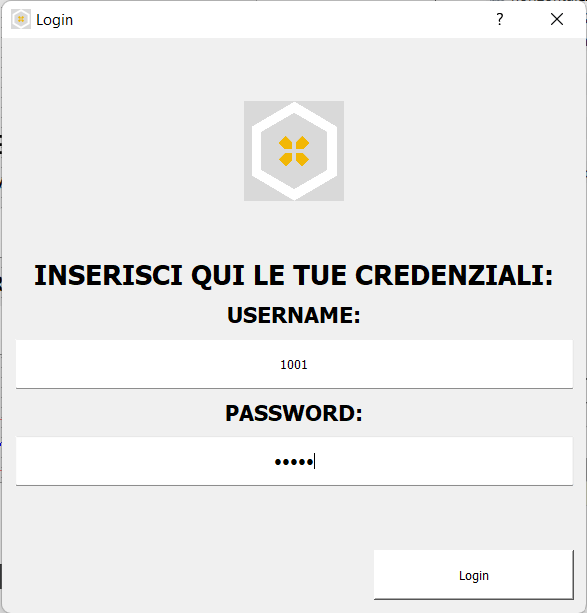
\includegraphics[width=0.4\linewidth]{./ImageFiles/loginform}
	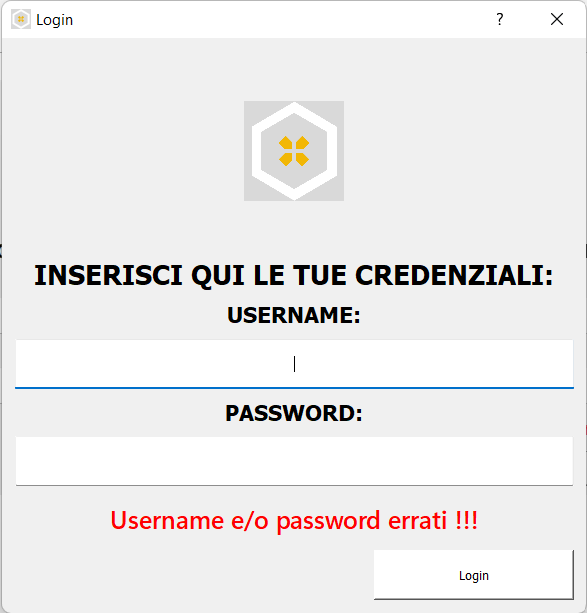
\includegraphics[width=0.4\linewidth]{./ImageFiles/loginform_errato}
	\caption{Finestra di login e login errato.}
	\label{fig:loginform}
\end{figure}

Al contrario, se le credenziali di accesso sono corrette viene mostrato all'utente la schermata principale (\Fig\ref{fig:home_foreman}). La schermata principale è divisa in due sezioni. Nella parte sinistra è possibile vedere tutte le informazioni memorizzate dell'utente (fotografia, matricola, nome, cognome, data di nascita, email, numero di telefono, sesso) e le informazioni relative alla squadra (identificativo e nome della squadra, nome e coordinate dell'area di intervento). Le informazioni relative alla squadra non sono mostrate nel caso in cui l'utente sia un amministratore, in quanto non appartenente a nessuna squadra.

\begin{figure}[h!]
	\centering
	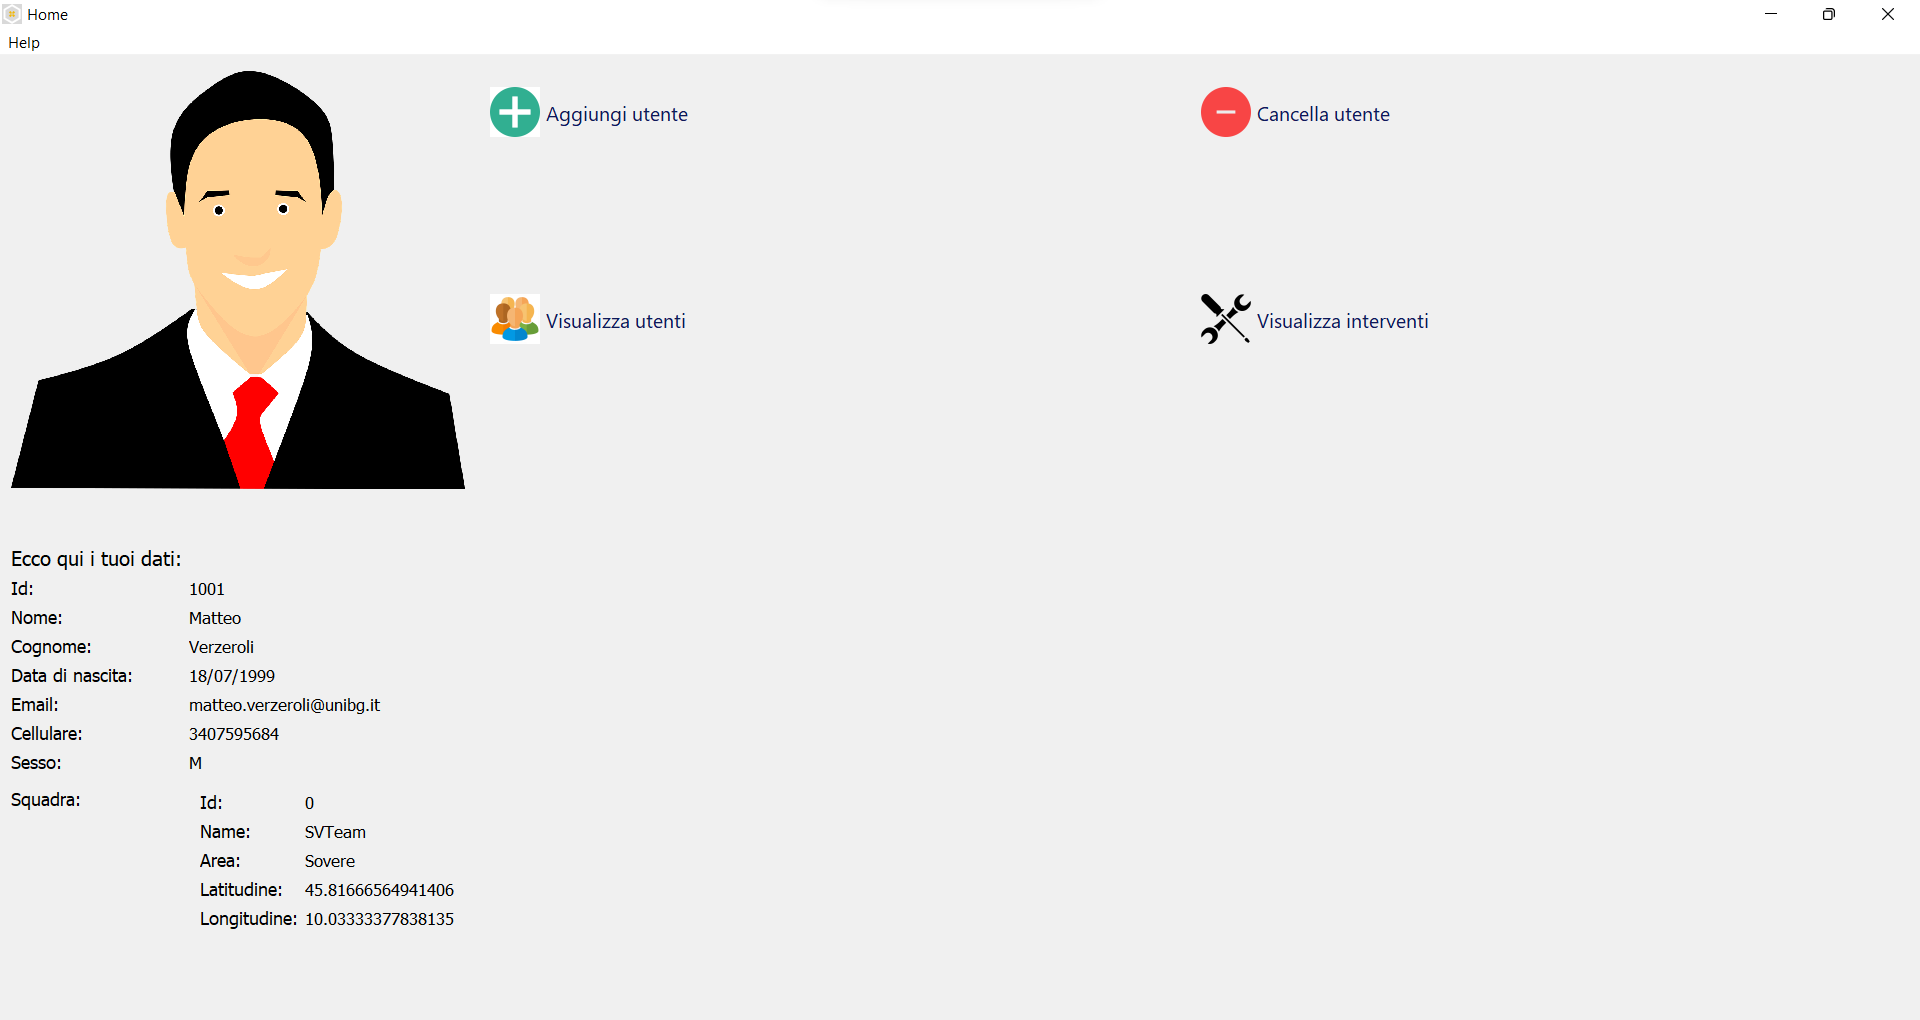
\includegraphics[width=1\linewidth]{./ImageFiles/home_foreman}
	\caption{Finestra principale di un caposquadra.}
	\label{fig:home_foreman}
\end{figure}

Nella parte destra è possibile vedere un piccolo menù dalla quale scegliere le operazioni da eseguire: aggiungere un utente, eliminare un utente, visualizzare gli utenti e gli interventi. A seconda del ruolo dell'utente loggato, questo menù mostrerà diverse opzioni. In particolare, al volontario è permesso solamente visualizzare gli interventi, mentre all'amministratore non è possibile visualizzare gli interventi. Cliccando un pulsante nel menù sarà possibile eseguire le operazioni richieste.

\subsection{Inserimento nuovo utente}
Cliccando su \textit{Aggiungi utente} viene visualizzata una form da compilare per inserire i dati dell'utente da inserire, come mostrato nella \Fig\ref{fig:new_user}. 
\begin{figure}[h!]
	\centering
	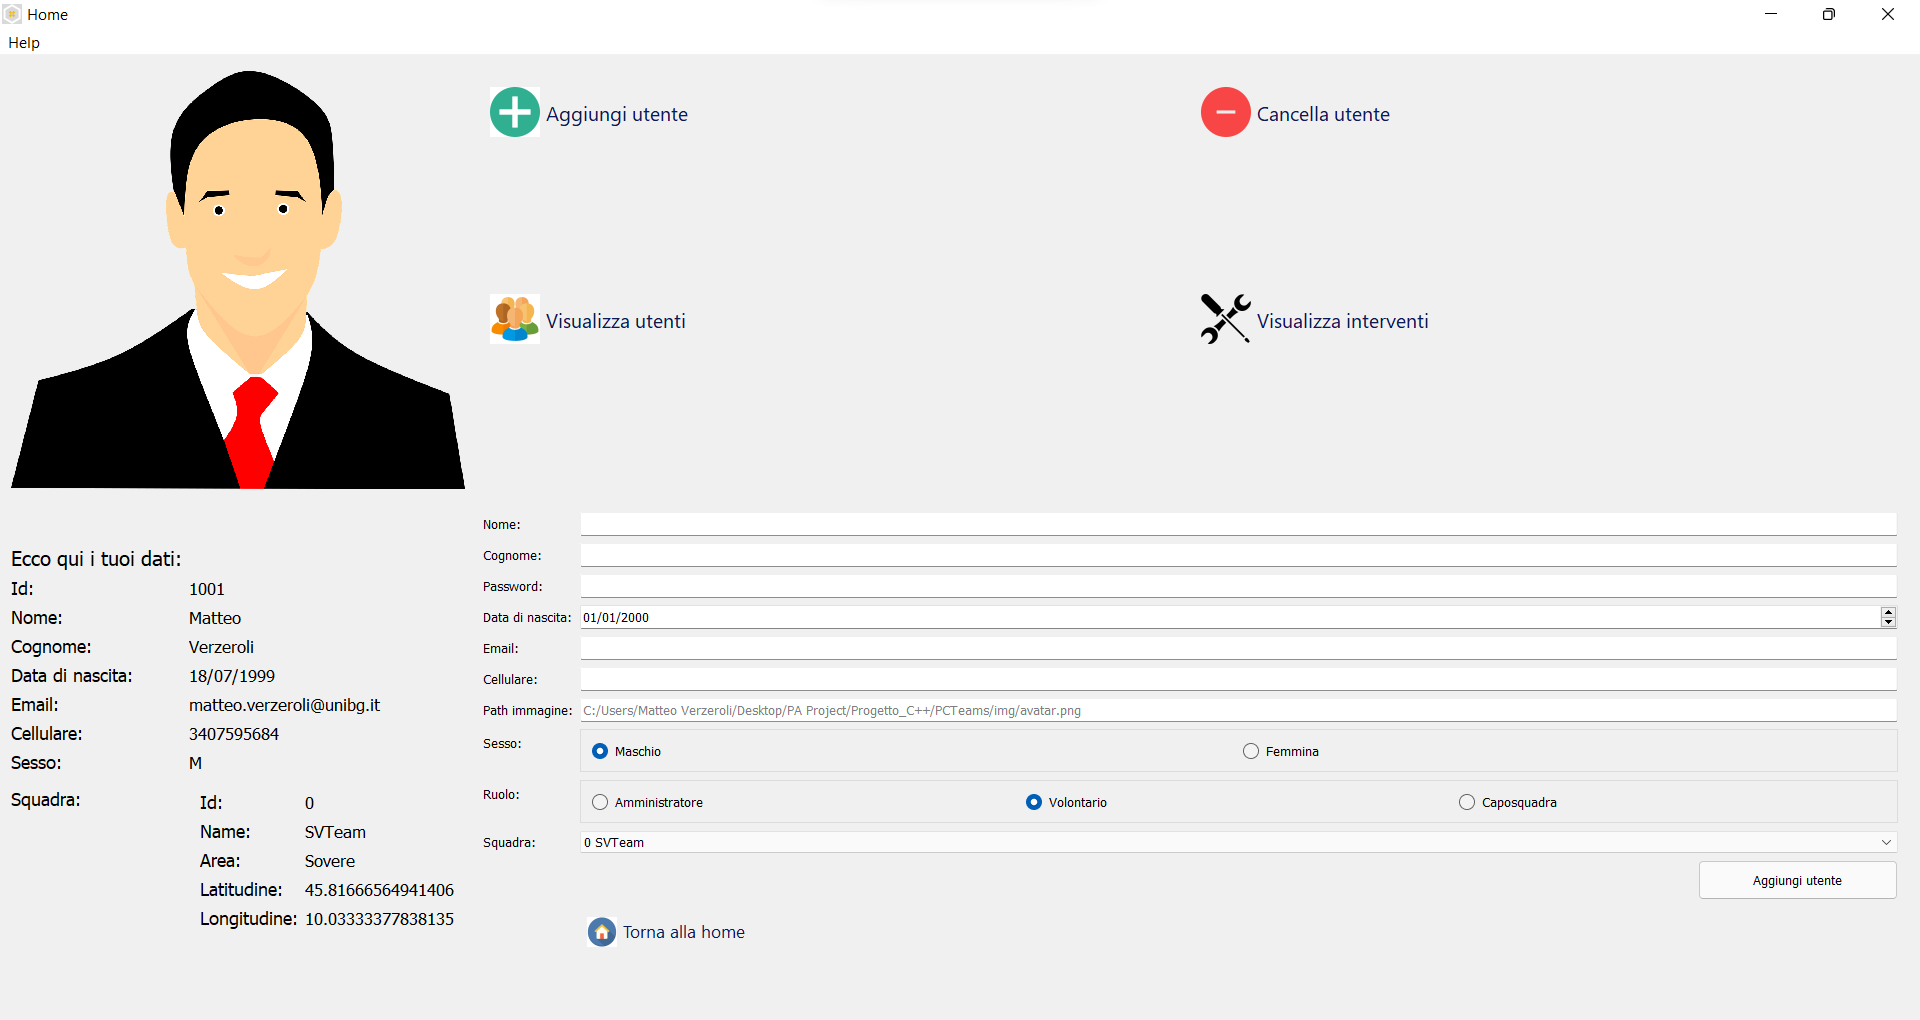
\includegraphics[width=1\linewidth]{./ImageFiles/new_user}
	\caption{Inserimento nuovo utente.}
	\label{fig:new_user}
\end{figure}

Si noti in particolare che bisogna anche indicare il ruolo. Se viene cliccato il ruolo \textit{Volontario} oppure \textit{Caposquadra}, viene mostrato anche una \textit{combo box} nella quale è possibile scegliere una squadra in cui inserire un utente.

Nel caso in cui si voglia inserire un volontario, le squadre selezionate vengono così selezionate: 
\begin{itemize}
	\item se l'utente attualmente loggato è un amministratore, vengono mostrate tutte le squadre inserite nel sistema;
	\item se l'utente attualmente loggato è un caposquadra, viene mostrata solamente la propria squadra.
\end{itemize}
Invece, se si vuole inserire un caposquadra vengono mostrate tutte le squadre inserite nel sistema che non hanno ancora un caposquadra.
Premendo il pulsante \textit{Inserisci utente}, l'utente viene inserito nel sistema e viene mostrato un messaggio di conferma nella \textit{status bar} in fondo alla finestra. Se non vengono compilati tutti i campi, il sistema segnala finestra di errore (\Fig\ref{fig:new_user_error}). 

\begin{figure}[h!]
	\centering
	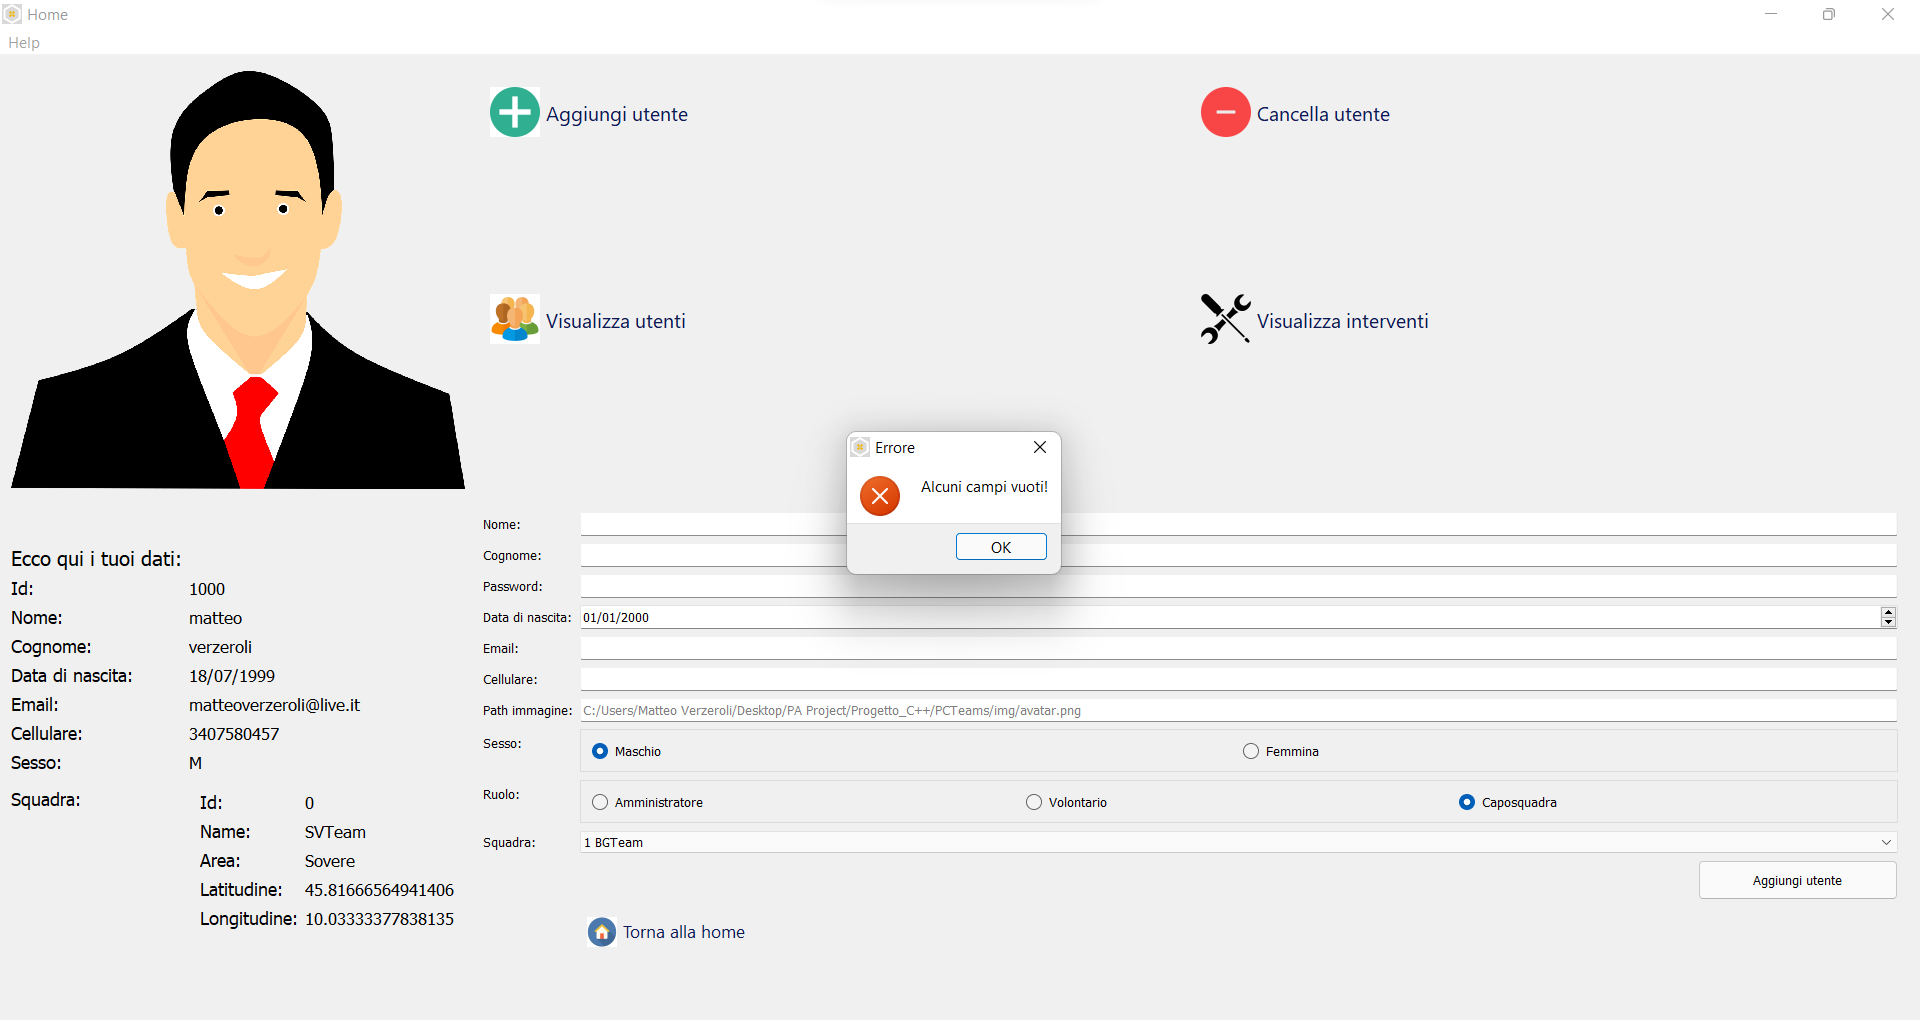
\includegraphics[width=1\linewidth]{./ImageFiles/new_user_error}
	\caption{Errore inserimento nuovo utente.}
	\label{fig:new_user_error}
\end{figure}

\subsection{Cancella utente}
Nel caso in cui si voglia cancellare un utente, è possibile selezionare una squadra (tramite una \textit{combo box}) e indicare l'utente da eliminare, selezionandolo nella lista sottostante (\Fig\ref{fig:delete_user}). Un caposquadra può solamente cancellare utenti della propria squadra. Un amministratore invece può eliminare utenti da tutte le squadre, compresi gli amministratori. Nessuno può eliminare se stesso. Infatti, in tal caso viene mostrato un messaggio di errore.

\begin{figure}[h!]
	\centering
	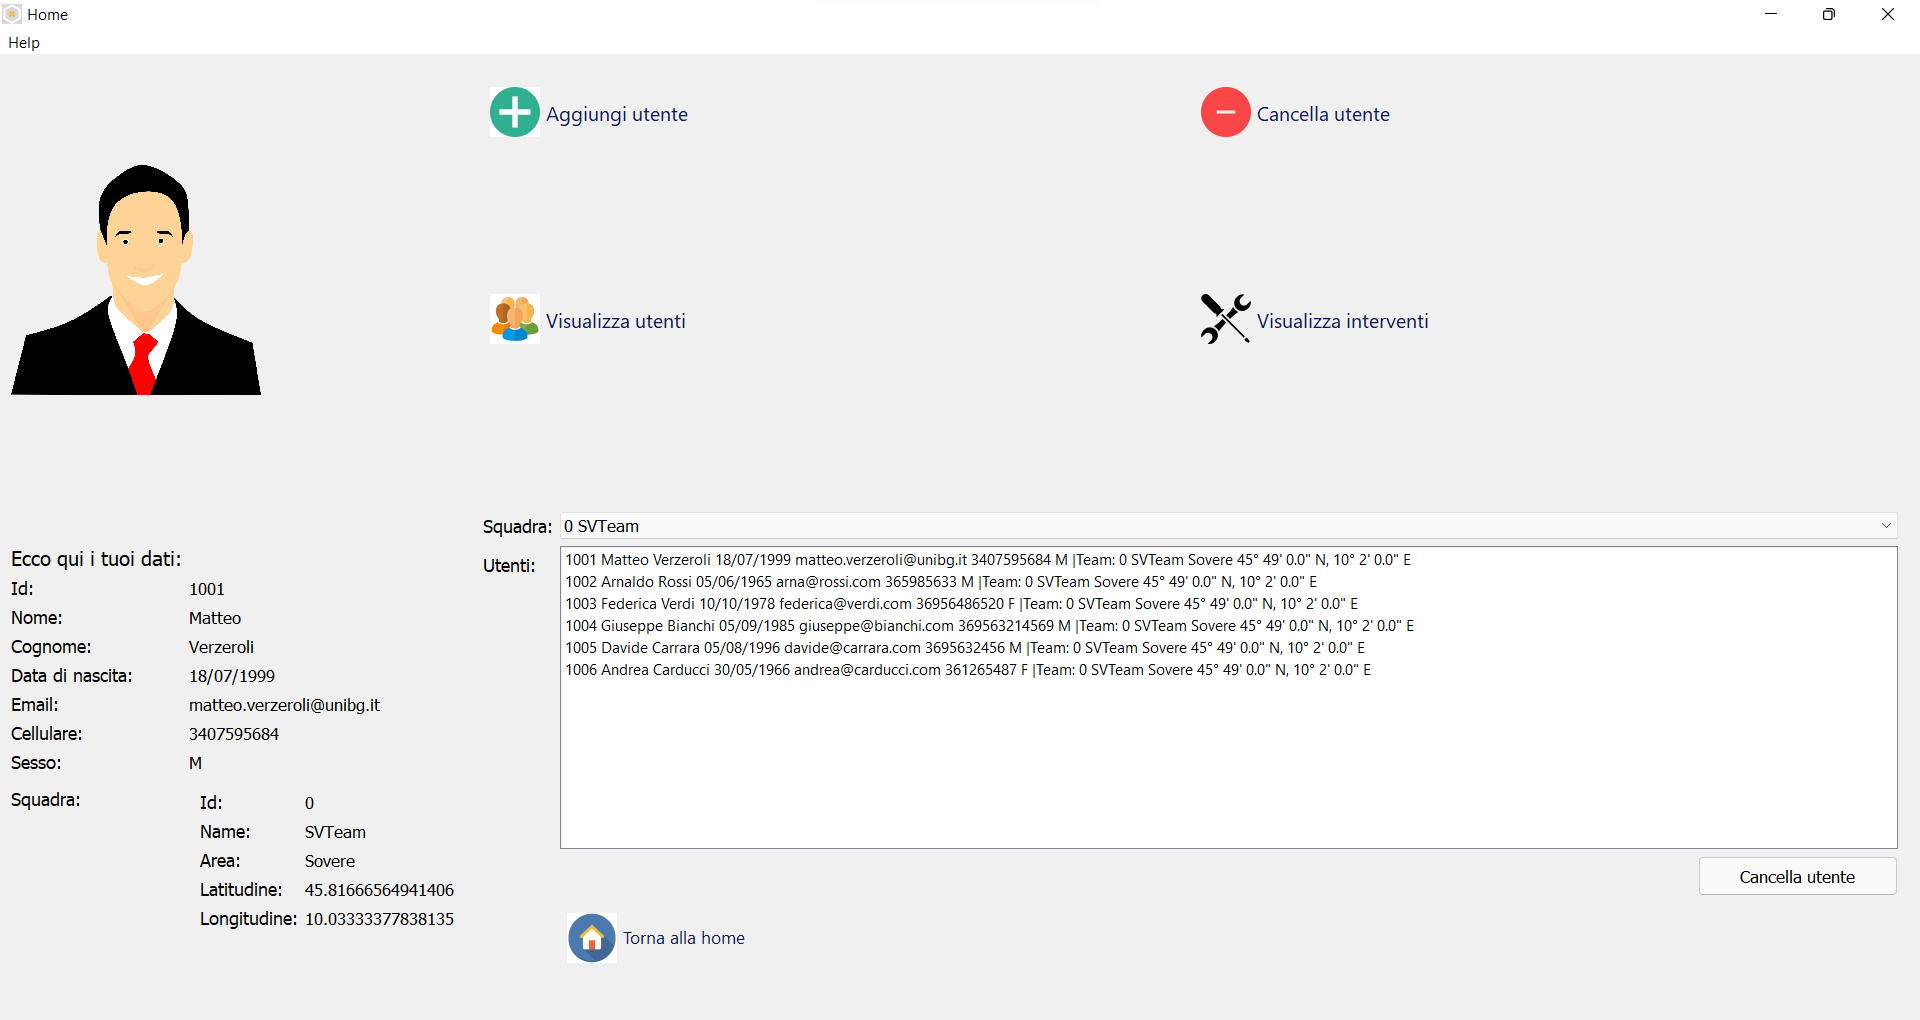
\includegraphics[width=1\linewidth]{./ImageFiles/delete_user}
	\caption{Cancellazione utente.}
	\label{fig:delete_user}
\end{figure}

\subsection{Visualizza utenti}
Un caposquadra o un amministratore possono visualizzare gli utenti appartenenti a una squadra (\Fig\ref{fig:view_user}), selezionandola dalla \textit{combo box}. `E possibile visualizzare gli amministratori. Per questa funzionalità, se l'utente loggato è un amministratore potrà visualizzare la lista degli utenti appartenenti a tutte le squadre inserite nel sistema. Al contrario, se è un caposquadra potrà vedere solamente gli amministratori o la propria squadra.

\begin{figure}[h!]
	\centering
	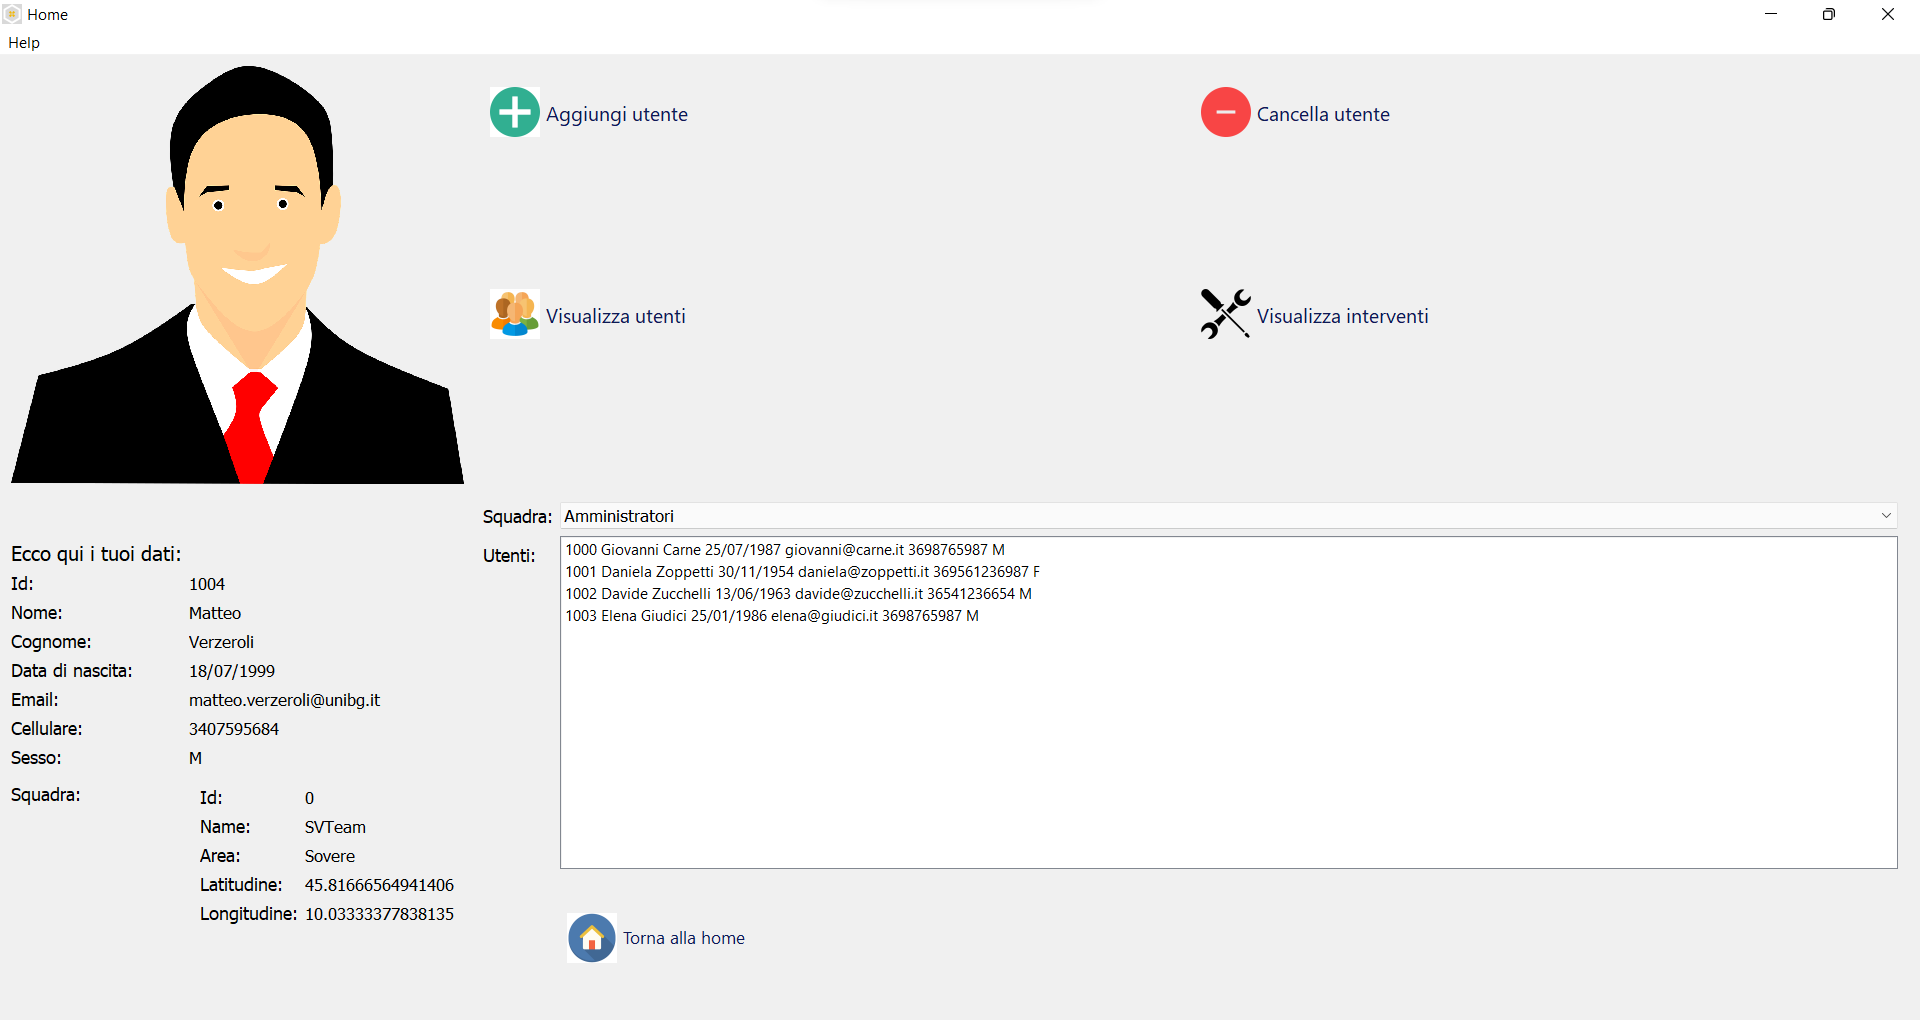
\includegraphics[width=1\linewidth]{./ImageFiles/view_user}
	\caption{Visualizzazione utenti.}
	\label{fig:view_user}
\end{figure}

\subsection{Visualizza interventi}
I volontari e i capisquadra possono visualizzare rispettivamente gli interventi della propria squadra oppure di tutte le squadre. Cliccando su \textit{Visualizza interventi}, viene mostrato un calendario sul quale selezionare una data (\Fig\ref{fig:view_operation}). Vengono cosi mostrati gli interventi programmati in quella giornata. Gli eventi possono essere creati solo dal caposquadra, cliccando sul pusante \textit{Inserisci un nuovo intervento}.
\begin{figure}[h!]
	\centering
	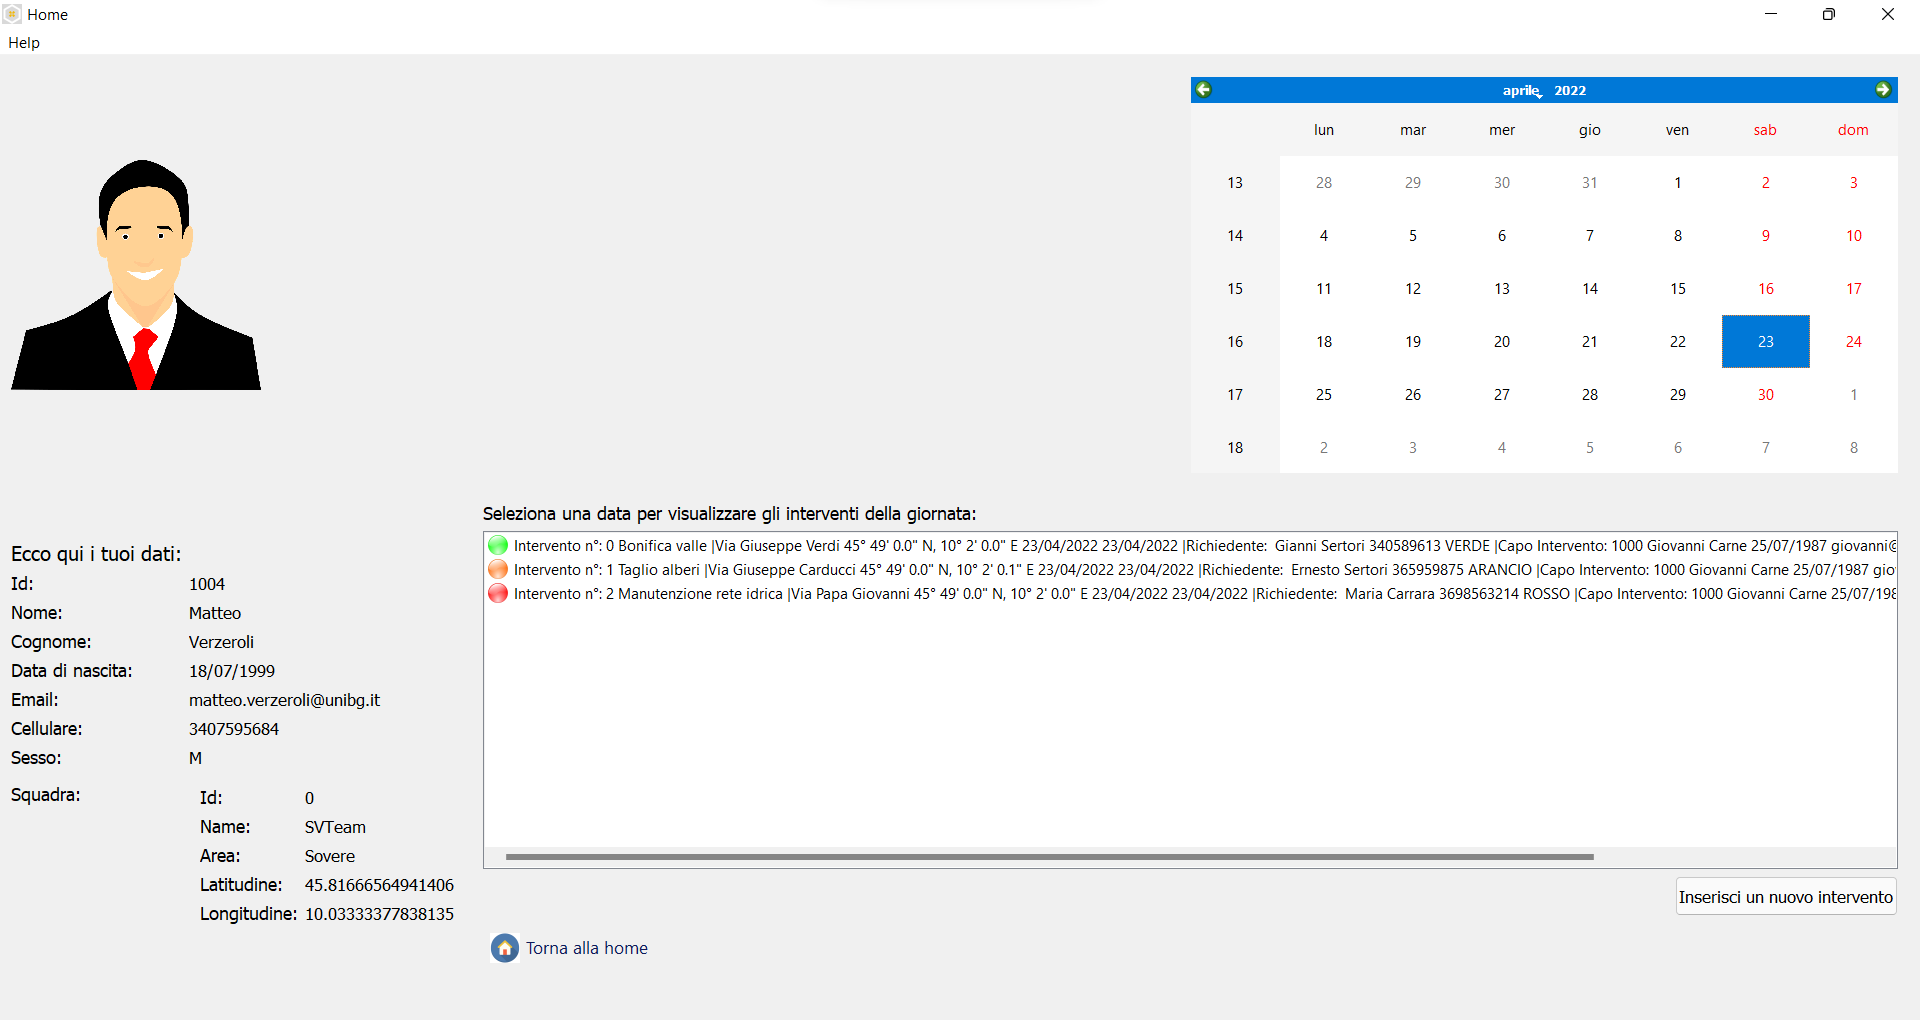
\includegraphics[width=1\linewidth]{./ImageFiles/view_operation.png}
	\caption{Visualizzazione interventi.}
	\label{fig:view_operation}
\end{figure}

Quando il pulsante viene cliccato, viene mostrata una form per l'inserimento delle informazioni dell'intervento, come mostrato in figura \ref{fig:new_op}. Cliccando su \textit{Inserisci intervento} un messaggio di conferma indica che l'evento è stato inserito. Se tutti i campi non sono stati completati, viene invece mostrato un messaggio di errore.

\begin{figure}[h!]
	\centering
	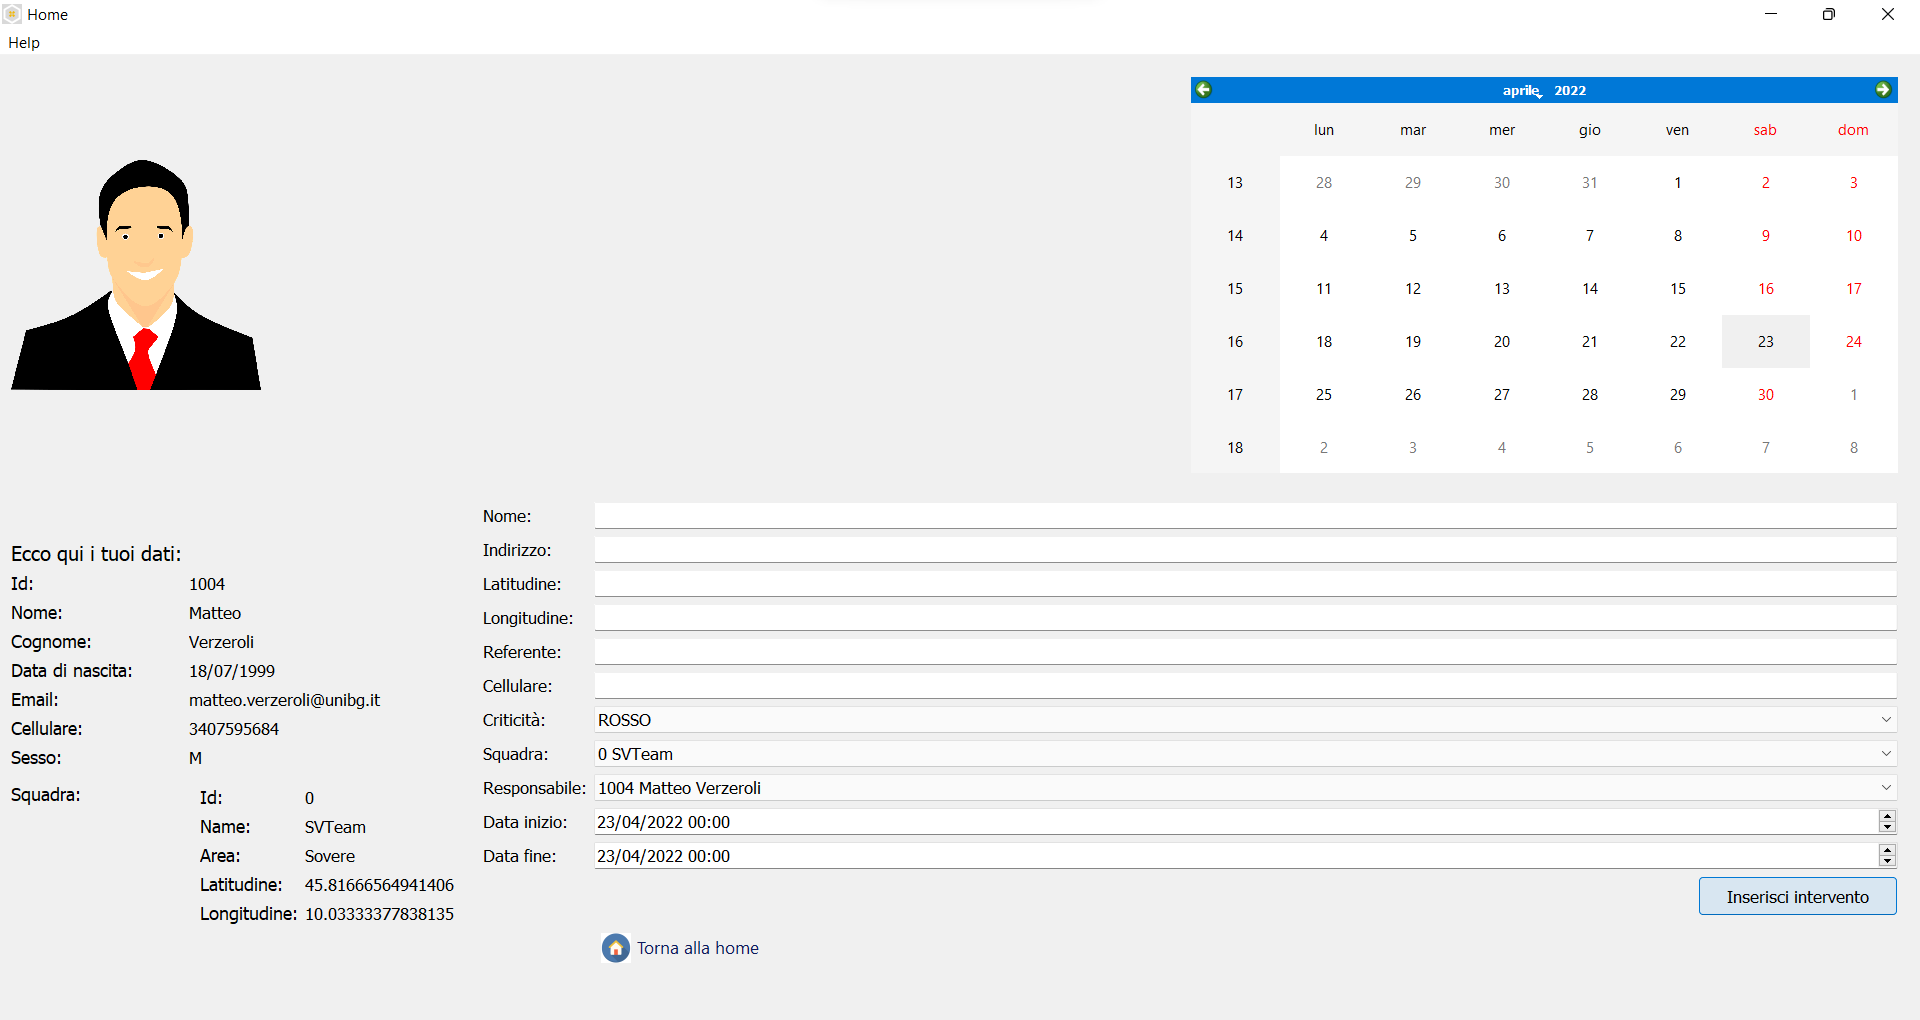
\includegraphics[width=1\linewidth]{./ImageFiles/new_op.png}
	\caption{Inserimento nuovo intervento.}
	\label{fig:new_op}
\end{figure}

\subsection{Lougout}
Cliccando nel menù in alto alla schermato \textit{Help}, è possibile effettuare il logout. Viene quindi mostrata la finestra di login.

\begin{landscape}
	\section{Diagramma delle classi}
	\begin{figure}[h!]
		\centering
		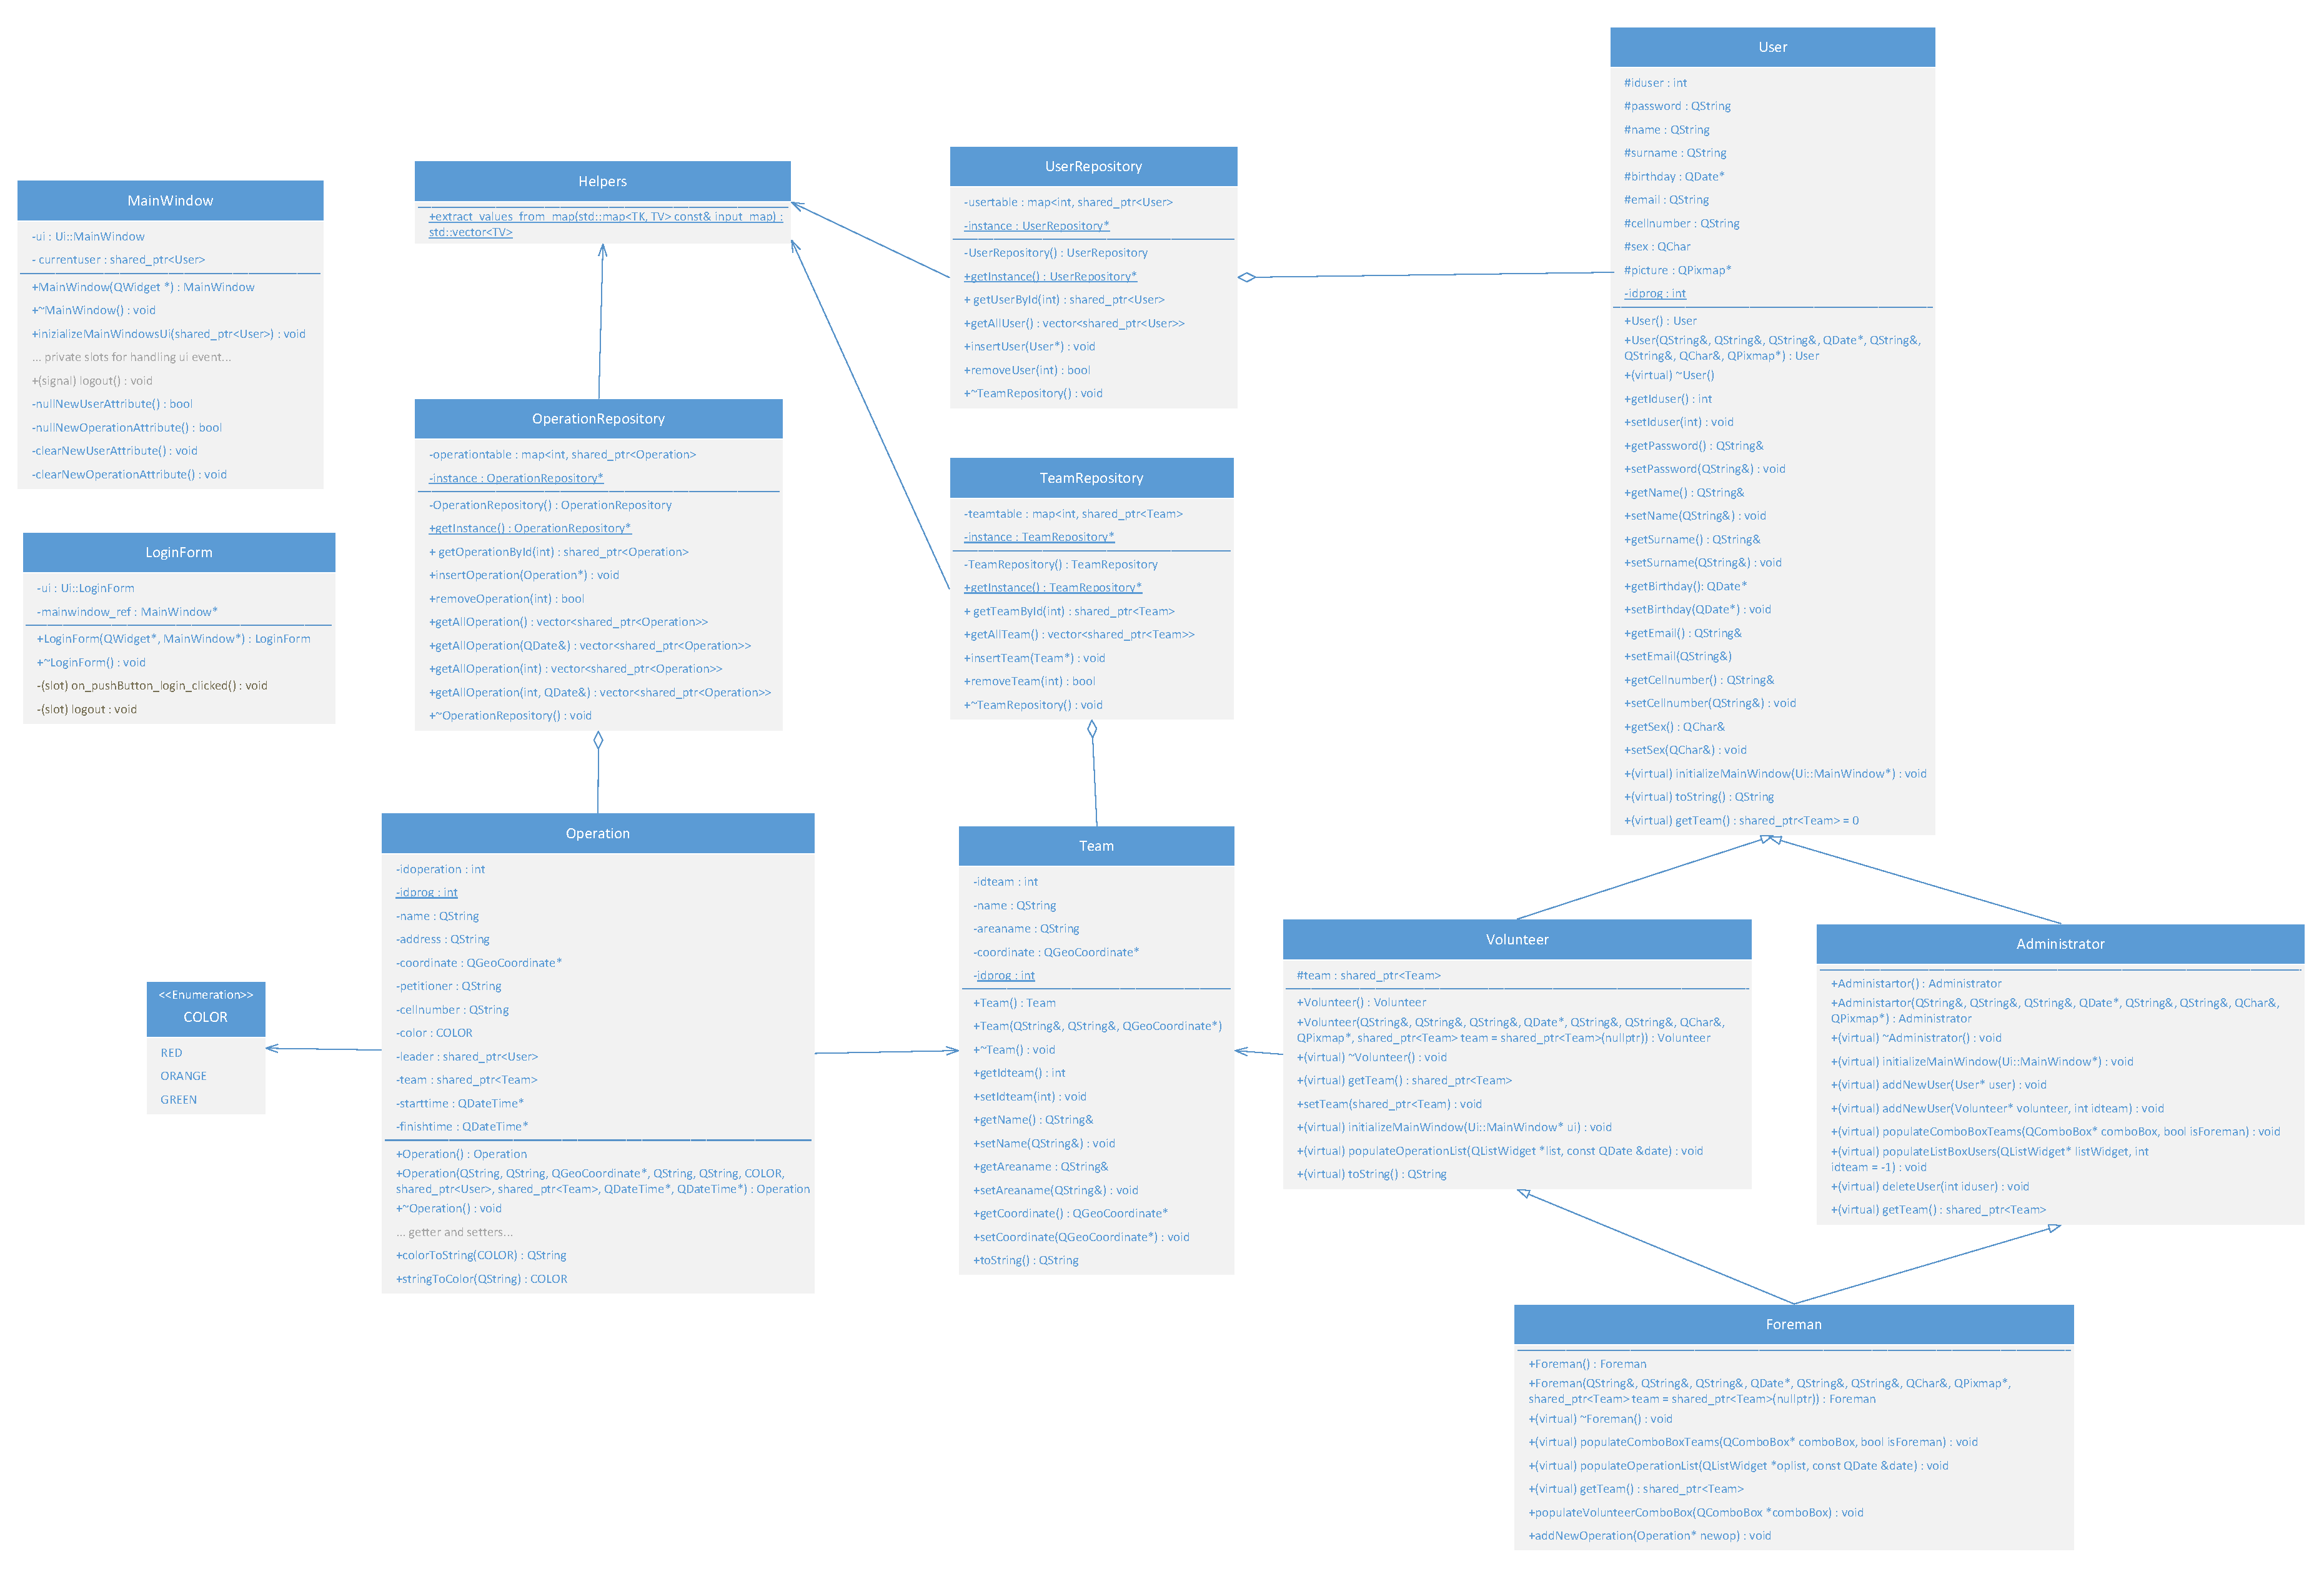
\includegraphics[width=0.9\linewidth]{./OtherFiles/Class Diagram}
		\caption{Class Diagram.}
		\label{fig:class_diagram}
	\end{figure}
\end{landscape}

\section{Dettagli implementazione}
L'\textit{entry point} dell'applicazione sviluppata è la funzione \textit{main} definita nel file \texttt{main.cpp}. All'interno del main vengono create le istante dell'applicazione, della finestra della \textit{Home} e del \textit{Login}. Infine, vengono creati alcuni utenti, squadre e operazioni per poterli utilizzare come esempio, e viene lanciata l'applicazione. Le finestre sono realizzate tramite i \textit{QWidgets} offerti da Qt e sono descritte nei file \texttt{.ui}. Ogni finestra (MainWindow che rappresenta la home e LoginForm che rappresenta la pagina di login) è descritta da una classe, implementata nei file \texttt{.h} (header) e \texttt{.cpp}. All'interno di queste classi, sono definiti gli \textit{slots}, tipiche del linguaggio Qt, che rappresentano degli \textit{event handler} degli eventi sollevati dall'interfaccia grafica (o da altre classi). In questo caso, entrambe le classi derivano dalla classe \textit{QObject}, che integra alcune funzioni base utili per lo sviluppo in Qt.

\subsection{Ereditarietà multipla}
Gli utenti sono rappresentati tramite una gerarchia di classi, che ne permette la differenziazione in base al ruolo. In particolare, la classe base è rappresentata dalla classe \texttt{User}, astratta in quanto contiene un metodo \textit{pure virtual}. Da questa derivano, in modo virtuale, la classe \texttt{Volunteer} e \texttt{Administator}. Infine, la classe \texttt{Foreman}, che rappresenta il caposquadra, deriva sia da \texttt{Volunteer} che da \texttt{Administator}. Si va quindi a costituire una struttura a \textit{diamante}, che porterebbe a problemi negli oggetti di tipo \texttt{Foreman}, che conterrebbero due differenti istanze di \texttt{User}: una ereditata da \texttt{Volunteer} e una da \texttt{Administrator}. Il \textit{problema del diamante} si risolve utilizzando l'ereditarietà virtuale da \texttt{User} da parte delle classi \texttt{Volunteer} e \texttt{Administator}.

\lstinputlisting[language=C++]{./OtherFiles/virtual_inheritance.cpp}

\subsection{Distruttore virtual}
Tutti i distruttori delle classi che ammettono sottoclassi sono stati dichiarati \textit{virtual}, in modo tale che la distruzione di un oggetto puntato da un riferimento della superclasse richiami in modo corretto i distruttori delle sottoclassi.
\lstinputlisting[language=C++]{./OtherFiles/virtual_destructor.cpp}

\subsection{Metodo pure virtual}
La classe \texttt{User} è definita astratta a causa della presenza di un metodo \textit{pure virtual}. Per cui, non è possibile creare una istanza del tipo \texttt{User}. Questo metodo, deve essere quindi ridefinito in ogni sottoclasse.
\lstinputlisting[language=C++]{./OtherFiles/pure_virtual.cpp}

\subsection{Metodi virtual: overriding}
Alcuni metodi sono stati definiti virtual, in modo da poter utilizzare il polimorfismo offerto dal linguaggio tramite l'utilizzo di riferimenti agli oggetti. Ad esempio:
\lstinputlisting[language=C++]{./OtherFiles/virtual_method.cpp}
Questo metodo è stato implementato nella classe \texttt{User} e in tutte le sottoclassi e si occupa di inizializzare la finestra \textit{Home} in base al ruolo dell'utente autenticato.

\subsection{Overload di metodi}
In alcuni casi, si è eseguito l'overload dei metodi, definendo diverse funzioni con lo stesso nome ma differente segnatura, in modo da differenziarne il comportamento in base ai parametri passati. Ad esempio:
\lstinputlisting[language=C++]{./OtherFiles/method_overload.cpp}

\subsection{Pattern Singleton}\label{sec:singleton}
Le classi \texttt{UserRepository}, \texttt{TeamRepository} e \texttt{OperationRepository} rappresentano delle tabelle (costituite da \textit{mappe chiave-valore}) nelle quali vengono salvate le informazioni relative rispettivamente a utenti, squadre e interventi, simulando le operazioni di un \textit{database}. Per garantire l'unicità di ogni \textit{repository}, queste classi sono state definite secondo il pattern \textit{Singleton}, definendo il costruttore privato. In questo modo non è possibile creare istanze della classe al di fuori della stessa. Tuttavia, è possibile accedere all'istanza tramite il metodo \textit{getInstance()}, che restituisce un puntatore all'istanza della classe. In questo modo, si può accedere ad alcuni metodi per eseguire operazione sulla tabella che conserva i dati. Si riporta di seguito la definizione della classe \textit{UserRepository}:
\lstinputlisting[language=C++]{./OtherFiles/userrepository.cpp}

\subsection{STL: std::vector, std::map, std::iterator}
All'interno dell'applicazione sono stati utilizzati i \textit{containers} \texttt{vector} e \texttt{map} forniti dalla \textit{Standard Template Library}. In particolare, le classi descritte nella sezione \ref{sec:singleton}, memorizzano utenti, squadre e interventi utilizzando una mappa \textit{chiave-valore}, in cui la chiave è di tipo \texttt{int} (costituita dall'id dell'oggetto) mentre il valore è uno \textit{smart pointer} all'oggetto. Ad esempio, la mappa che permette la memorizzazione degli utenti è stata dichiarata nel seguente modo:
\lstinputlisting[language=C++]{./OtherFiles/map.cpp}
Si è scelto di utilizzare una mappa per rendere efficiente le operazioni di ricerca tramite l'id dell'utente. Per permettere il polimorfismo (ossia memorizzare oggetti delle sottoclassi del tipo \texttt{User}), evitando il fenomeno dello \textit{slicing}, è stato necessario definire il \textit{valore} della mappa come puntatore di tipo \texttt{User}. Inoltre, affinché fosse garantita la distruzione corretta dell'oggetto puntato, si sono utilizzati i puntatori smart di tipo \textit{shared}, descritti nella sezione successiva. In questo modo, quando viene cancellato dalla mappa il riferimento alla risorsa, viene chiamato il distruttore dell'oggetto (se non sono più attivi altri riferimenti).

In alcuni casi, sono stati utilizzati anche oggetti di tipo \textit{vector}, che permettono la definizione di una lista di oggetti. Ad esempio, si riporta la definizione del metodo che restituisce tutti gli utenti inseriti nel sistema:
\lstinputlisting[language=C++]{./OtherFiles/vector.cpp}

Per scorrere vettori e mappe sono stati usati gli iteratori, sempre forniti dalla STL:
\lstinputlisting[language=C++]{./OtherFiles/iterators.cpp}

\subsection{Smart pointers: shared\textunderscore ptr} 
Nel progetto realizzato, si sono spesso utilizzati degli \textit{smart pointers} per semplificare l'utilizzo di puntatori agli oggetti. Inoltre, i puntatori intelligenti permettono di evitare problemi quali \textit{dengling pointers} e \textit{memory leak}, tipici dell'utilizzo non corretto dei puntatori. In particolare, si sono utilizzati gli \texttt{shared\textunderscore ptr<...>}, che permettono proprietari multipli del puntatore raw sottostante. In questo modo, possono essere copiati e passati come parametri ai metodi.
\lstinputlisting[language=C++]{./OtherFiles/smartpointers.cpp}

\subsection{Template}
In molte occasioni, si sono utilizzati i \textit{template}, come ad esempio la definizione del tipo degli \textit{smart poiter}, delle mappe e dei \textit{vector} creati. Nella classe \texttt{Helpers} si è anche scritto un metodo che restituisce un vettore di tutti i valori contenuti nella mappa, passata come argomento. Affinché questo metodo fosse generico per ogni tipo di mappa chiave-valore, si è scelto di implementarlo utilizzando i \textit{template} nel seguente modo:
\lstinputlisting[language=C++]{./OtherFiles/template.cpp}

\subsection{Enum}
All'interno dell'applicazione si è inoltre definito un tipo \texttt{enum} per rappresentare la criticità di un intervento, definendolo nel seguente modo:
\lstinputlisting[language=C++]{./OtherFiles/enum.cpp}
Sono stati poi inseriti dei metodi statici nella classe \texttt{Operation} per gestire l'utilizzo della enumerazione.

\subsection{Friend}
A scopo di debug, è stato definito l'operatore \textit{<<} per gli oggetti di tipo \texttt{User}. Dal momento che si accedeva ai membri privati della classe, la definizione è stata dichiara friend nel modo seguente:
\lstinputlisting[language=C++]{./OtherFiles/friend.cpp}
